

Despite the growing popularity of more sophisticated deep learning-based embedding models, here we leverage latent dirichlet allocation (i.e., topic modeling) to embed episode and recall text.  This decision was motivated by several factors.  First, topic models capture the \textit{essence} of a text passage devoid of the specific set and order of words used.  This was an important feature of our model since different people may accurately recall a scene using very different language. Second, words can mean different things in different contexts (e.g. ``bat'' may be the act of hitting a baseball, the object used for that action, or as a flying mammal).  Topic models are robust to this, allowing words to exist as part of multiple topics.  Last, topic models provide a straightforward means of recovering the weights for the particular words comprising a topic, enabling straightforward interpretation of an event's contents (e.g. Fig.~\ref{fig:topics}). Other models such as the Universal Sentence Encoder, GPT-2, and GPT-3 offer context-sensitive encoding of text passages, but the encoding space is complex and non-linear, and thus recovering the original words used to fit the model is not straightforward. However, it is worth pointing out that our general framework is divorced from the particular choice of language model. Moreover, many of the aspects of our framework could be swapped out for other choices. For example, the language model, the timeseries segmentation model and the episode-recall matching function could all be customized to suit a particular question space or application. Indeed for some questions, recovery of the particular words used to describe a memory may not be necessary, and thus other text-modeling approaches (including the deep learning-based embedding models described above) may be preferable. Future work will explore the influence of particular model choices on the framework's efficacy.

In extending classical free recall analyses to our naturalistic memory framework, we recovered two patterns of recall dynamics central to list-learning studies: a heightened probability of initiating recall with the first presented ``item'' (in our case, episode events; Fig.~\ref{fig:list-learning}A) and a strong bias toward transitioning from recalling a given event to recalling the one immediately following it (Fig.~\ref{fig:list-learning}B).  However, equally noteworthy are the typical free recall results \textit{not} recovered in these analyses, as each highlights a fundamental difference between the list-learning paradigm and naturalistic memory paradigms like the one employed in the present study.  The most noticeable departure from hallmark free recall dynamics in these findings is the apparent lack of a serial position effect in Figure \ref{fig:list-learning}C, which instead shows greater and lesser recall probabilities for events distributed across the episode.  Stimuli in free recall experiments most often comprise lists of simple, common words, presented to participants in a random order. \citep[In fact, numerous word pools have been developed based on these criteria; e.g.,][]{FrieEtal82}.  These stimulus qualities enable two assumptions that are central to word list analyses, but frequently do not hold for real-world experiences.  First, researchers conducting list-learning studies may assume that the content at each presentation index is essentially equal, and does not possess attributes that would render it, on average, more or less memorable than others.  Such is rarely the case with real-world experiences or experiments meant to approximate them, and the effects of both intrinsic and observer-dependent factors on stimulus memorability are well established \citep[for review see][]{ChunTurk07, ByliEtal15, TyngEtal17}.  Second, the random ordering of list items ensures that (across participants, on average) there is no relationship between the thematic similarity of individual stimuli and their presentation positions---in other words, two successively presented items are no more likely to be highly semantically similar than they are to be highly dissimilar.  In most cases, the exact opposite is true of real-world episodes.  Our internal thoughts, our actions, and the physical state of the world around us all tend to follow a direct (often causal) progression.  As a result, each moment of our experience tends to be inherently more similar to surrounding moments than to those in the distant past or future.  Memory literature has termed this strong temporal autocorrelation ``context,'' and in various media that depict real-world events (e.g., movies or written stories), we recognize it as a \textit{narrative structure}.  While a random word list (by definition) has no such structure, the logical progression between ideas and actions in a naturalistic stimulus prompts the rememberer to recount presented events in order, starting with the beginning.  This tendency is reflected in our findings' second departure from typical free recall dynamics: a lack of increased probability of first recall for end-of-sequence events (Fig.~\ref{fig:list-learning}A).

Because they disregard presentation order-dependent variability in the stimulus content, analyses such as those in Figure \ref{fig:list-learning} enable a more sensitive analysis of presentation order-dependent temporal dynamics in free recall. Yet by the same token, they paint a wholly incomplete picture of memory for naturalistic episodes.  In an attempt to address this shortcoming, we have developed a framework in the present study that characterizes the explicit semantic content of the stimulus and subsequent recalls.  However, sensitivity to stimulus and recall content introduces a new challenge: distinguishing between levels of recall quality for a stimulus (e.g., an event) that is considered to have been ``remembered.''  When modeling memory in an experimental setting, recall quality for individual events is often cast as binary (e.g., a given list item was simply either remembered or not remembered).  Various models of memory (e.g., \citealp{Yone02}) attempt to improve upon this by including confidence ratings, rendering this binary judgement instead categorical.  To better evaluate naturalistic memory quality, we introduce a continuous metric (\textit{precision}), which reflects the level of completeness of a participant's recall for a feature-rich experience.  Additionally, recall quality for a single event is typically assessed independently from that for all other events (e.g., it is difficult to ``compare'' a participant's binary recall success for list item 1 to that of list item 10).  The second novel metric we introduce (\textit{distinctiveness}) is based on analyzing of the correlational structure of an individual's full set of recall events, and reflects the specificity of their memory for a single experienced event.  We find that both of these metrics relate to the overall number of episode events participants successfully recalled, and that our precision metric additionally relates to \cite{ChenEtal17}'s hand-annotated memory memory scores.

We did not find evidence that participants' average recall distinctiveness was related to their hand-annotated memory scores computed by~\cite{ChenEtal17}.  One possible explanation is that, in hand-scoring each participant's verbal recall for each of 50 (manually-deliniated) scenes, ``[a] scene was counted as recalled if the participant described any part of the scene''~\citep{ChenEtal17}.  In other words, both an extensive description of a scene's content and a brief mention of some subset of its content were (binarily) considered equally successful recalls.  By contrast, we identify the event structure in participants' recalls in an unsupervised manner, independent of the episode event-timeseries, prior to mapping between episode and recall content.  Our HMM-based event-segmentation produces boundaries between timepoints where the topic proportions shift in a substantial way, and because a small handful of words is unlikely to contribute significantly to the topic proportions for any sliding window, such brief scene descriptions will most often not result in a sufficiently large shift in the resulting topic proportions for the HMM to identify an event boundary.  Instead, they will be grouped with a neighboring event, consequently lowering that event's distinctiveness score and by extension, the participant's overall distinctiveness score.  This is in essence the qualitative difference between distinctive and indistinctive recall, and reflects the comparison shown in Figure \ref{fig:distinctiveness-detail}C.  Intriguingly, prior studies show that pattern separation, or the ability to cleanly discriminate between similar experiences, is impaired in many cognitive disorders as well as natural aging \citep{StarEtal10, YassEtal11c, YassStar11b}.  Future work might explore whether and how these metrics compare between cognitively impoverished groups and healthy controls.

In the analyses outlined in Figure \ref{fig:brainz}, we identified two networks of brain regions whose responses during episode viewing were consistent with the temporal structure of the episode and recall topic trajectories, respectively. The network identified by the episode trajectory analysis included the ventromedial prefrontal cortex, left anterior temporal lobe, superior parietal and dorsal anterior cingulate cortex. The network from the episode-recall trajectory analysis also included the ventromedial prefrontal and superior parietal cortices, in addition to the posterior medial cortex (PMC) and the inferior temporal regions. Notably, \cite{ChenEtal17} also observed the PMC in a number of analyses including one that searched for regions whose activity patterns during encoding were reinstated during free recall. The PMC has been consistently identified in studies involving stimuli with meaningfully structured events~\citep{CohnRang17}. Further, the PMC is part of the "posterior medial" system, a network of brain regions thought to represent situation models~\citep{ZackEtal07} in support of memory, spatial navigation and social cognition~\citep{RangRitc12}. Given that we constructed our episode-recall searchlight model to capture temporal structure in the episode's semantic content (and how one's later recall aligns with that structure), we speculate that the PMC may play a role in constructing mnemonic events from meaningfully structured experiences.

Decoding the associated significance maps with \texttt{Neurosynth} revealed two intriguing results.  First, the top 10 terms returned for the episode-driven searchlight significance map were centered around themes of language and semantic meaning (Fig.~\ref{fig:brainz}).  In other words, the voxels identified as more reflective of the episode content's temporal structure (i.e., voxels with lower permutation correction-derived $p$-values), as defined by our model, were most likely to be reported as active in studies focused on the the neural underpinnings of semantic processing.  This finding is interesting, as our model specifically captures the temporal structure of the episode's \textit{semantic} content (e.g., as opposed to that of the visual, auditory, or affective content).  This suggests that the network of structures displayed in Figure \ref{fig:brainz}C may play a roll in processing the evolving semantic content of ongoing experiences.


Our second searchlight analysis identified a partially overlapping network of regions (Fig.~\ref{fig:brainz}D) whose patterns of activity as participants viewed the episode reflected the idiosyncratic structure of each individual's later recalls.  The associated significance map yielded a set of \texttt{Neurosynth} terms that primarily reflected names of specific structural regions (such as ``thalamus,'' ``anterior insula,'' ``anterior cingulate'' and ``inferior frontal''; Fig.~\ref{fig:brainz}).  Interestingly, these regions share membership in a common, large-scale functional network (termed the ``salience network'') involved in detecting and processing affective cues.  In particular, the latter three regions have been implicated in functions relevant to assigning personal meaning to an experience, including: ascribing subjective value to raw, sensory input \citep{MedfCrit10}; modulating semantic and phonological processing in response to personally salient stimuli \citep{KellEtal07b}; and directing and reallocating attention and working memory resources towards the most relevant stimuli \citep{MenoUddi10}.  This suggests that the network of structures displayed in Figure \ref{fig:brainz}D may be play a roll in transforming and restructuring ongoing experiences through the lens of one's prior experience and subjective emotions as they are encoded in memory.



%


Supplemental materials



trajectories obtained in the absence of a single feature and that of our original (i.e., full) model (Supp. Fig.~\ref{fig:feature-importance}A). First, we iteratively removed one transcribed feature from the scene descriptions and constructed a timepoints (1976) by topis (100) matrix using a topic model fit to the remaining features. We then represented the original model as well as the new model’s temporal structure as a timepoints-by-timepoints correlation matrix. Finally, we vectorized these correlation matrices and correlated them to each other resulting in a single number (for each feature removed from the model) representing the similarity of the ``feature-removed'' models to the full model.

In order to ascertain which features were important in relating the recall models to the video model, we similarly compared to the temporal structures of video and recall models deprived of a single feature at a time (Supp. Fig.~\ref{fig:feature-importance}B). For each feature removed, we transformed each participant’s recall transcript using a model trained on the feature-deprived video text windows (of 50 scene segments), and resampled the recall timeseries to match the shape of the video model (1976 timepoints). We then represented the temporal structures of each participant’s recall model as timepoints-by-timepoints correlation matrices and computed the average correlation with the temporal structure of the video model (across participants).





%METHODS


%Already say these in text:
\subsubsection*{Matching recall events to video events}


To estimate which video event each recall event referred to, we correlated the video events model and each recall events model. This resulted in a video events (34) by recall events (8-27) correlation matrix (for each participant) which contains the similarity between each video event and each recall event (see Fig.~\matchmats).  To find the most likely video event that a given recall event referred to, we computed the argmax over the columns of this matrix.  The result was a list of video event indices for each participant. These indices are analogous to the values found in a ``recall matrix'' from a free recall list learning experiment, but represent the recall of particular events (instead of words, for example).

\subsubsection*{Topic vector word clouds}
We created word clouds to visualize the themes contained in the recall events. One component of the topic model comprises a words (2117) by topics (100) matrix (R), where the rows represent the weight of a given word in each topic.  To find words that were maximally associated with a particular event vector, we computed the dot product between R and v, which gave a 1 by \# of words vector where the values represent the ``activation'' of each of in the event. Activation is defined as the weight of a particular word in a particular event. Then, we created word clouds by extracting the top $n$ words and plotting them where the size of the word is proportional to its activation in the event.

In the first analysis (Fig.~\ref{fig:topics}A,B), we quantified the most and least remembered topics/words throughout the entire video by computing a weighted average over all recall events, where the weights were proportional to memory for each recall event. To measure memory for each event, for each participant we computed the correlation between the video event vector and the closest recall event vector. We then averaged these correlation values across participants. We then computed a weighted average of all video events using the correlation values as weights. Next, we computed the dot product between this weighted-average video event vector and the R matrix (described in the paragraph above) to get activations for each word. Finally, we plotted the top 200 words where the size of the word is proportional to its activation. To get the least remembered topics/words, we performed the same analysis but inverted memory weights.

In the second analysis (Fig.~\ref{fig:topics}C), we created wordles for the top/bottom 3 remembered video events indexed by the average correlation values (Fig.~\ref{fig:topics}A).  To get the ``activations'' for words associated with the video events, we computed the dot product between the video event vector and the R matrix. The same procedure was used to get word activations for the recall events. We then plotted the top 200 words for the top/bottom 3 recalled events.


%%%%%

% DISCUSSION







% JRM THOUGHTS ON DISCUSSION:
% - Nature says "1-2 short paragraphs" -- needs to be much shorter.
% - I think we can get rid of anything we mention in the intro or results
% - Things not easily presented elsewhere are the background on the brain results and applications to education metrics.  I think we can focus on those two parts, add an "overview" and "conclusion" (potentially), and cut the rest.

Prior work on neural responses during naturalistic experiences and recall has largely focused on identifying brain regions whose responses are reliably similar across individuals ~\citep{LernEtal11, SimoEtal16, ChenEtal17, BaldEtal17, ZadbEtal17}. This allows one to identify which regions might be processing or representing the stimulus, or retrieving details of the experience during recall. Our approach is fundamentally different. We ask: which brain regions during video viewing match the video structure and how individual participants will recall the video later (in terms of the temporal correlations of their recall topic trajectory)? This latter approach highlights regions such as the medial prefrontal cortex (mPFC) and medial temporal lobes (MTL) that may respond in idiosyncratic ways across individuals, but that nonetheless play an important role in encoding experience into memory. In other work, the mPFC has been suggested to play a role in the representation of a ``schema'', or a network of prior knowledge that is consistent with the current task ~\citep{KestEtal12, GilbMarl17}. One interpretation for mPFC's involvement in our work is that mPFC represents participant-specific relationships with the content of the video, and its representation during scene viewing is related to how a participant later describes the scene. MTL activity patterns also matched participant's recall, which is consistent with a large body of literature highlighting the role of the MTL in episodic memory encoding ~\citep{PallWagn02, DavaEtAl03, RangEtal04, Dava06}.


%%%%

More broadly, these findings have strong implications for how we assess memory in other naturalistic contexts, such as the classroom or in a doctor's office.  Whereas academic tests often measure students' performance using metrics such as the proportion of correctly answered questions, our work suggests that this approach might ``miss the forrest for the trees''. We view ``true learning'' as understanding key concepts (i.e., understanding central themes in the learned content and how they relate) rather than regurgitating the greatest number of facts. In addition to educational contexts, our approach may provide unique metrics that can be used to assist in the diagnosis of memory disorders, and other psychiatric disorders that influence memory. For example, while the quantity of information recalled could be roughly matched between a healthy and patient population, and other aspects of the memory (such as the shape, serial order, precision or distinctiveness) might be different. Thus, this work serves as a foundation for more nuanced approaches to memory assessment that consider the trajectory and specific contents of memory for a naturalistic experience.


%%%%


Studying human memory is commonly distilled down to a process of matching specific moments of a past experience with specific mnemonic outcomes.  In traditional trial-based free recall experiments, individual stimuli encountered during encoding are typically labeled as ``remembered'' or ``forgotten'' depending on whether the stimulus is recalled/recognized during a subsequent test. While this approach has advanced our understanding of human memory immensely, it does not translate well to naturalistic experiences. For one thing, the contents of our recall at any given moment might be reflected in many prior experiences/moments. Furthermore, the particular words used to describe the experience will inevitably vary across people and even across repeated recollections within an individual. Thus, there is not a ``one-to-one'' mapping between naturalistic experiences and their mnemonic counterparts. For example, remembering the patterns and colors of each person's shirt in a crowd might be considered as excellent recall in a standard memory task setup. But if the rememberer failed to note that the people in the crowd were gathered for their surprise birthday party, then they would have missed the "point" of the experience.

Our topic modeling approach, whereby we consider the broad ``theme'' present in different moments of participants' experiences and their memories for those experiences, affords us the ability to flexibly and accurately characterize memory for naturalistic experiences. This approach allows us to quantify which moments from the past and the current recounted experience match in terms of their thematic content and critically, our ability to perform this matching does not require participants to use any specific overlapping words. Our work characterizes recollection of an experience by comparing the overall ``shape'' of a dynamic stimulus and a memory. We assess the quality of memory for the video participants viewed by measuring the match between the shapes of the video's trajectory and each participant's recall trajectory. By contrast, the number of recalls could be captured by the "sampling frequency" along that trajectory -- but the number of recalls alone cannot tell us whether participants successfully recollected the meaning of the story by capturing the salient points of the narrative that define its main shape. In addition to providing a way to capture the shape of an experience, this method affords the ability to quantify the particular contents of memory.  Whereas traditional approaches abstract over the content (e.g., percent correct), Our approach allows one to quantify which aspects of an experience are memorable and which fail to stick. This aspect of our approach opens the door for a much richer characterization of memory that considers not just how much information was recalled, but the particular details of that information as well.

An important question for future work concerns the factors that drive an individual to sample their recall trajectory finely or coarsely. For example, given a short recall interval, would participants intuitively gravitate towards coarser samplings that still outline the basic shape of the video's topic trajectory? Or if participants were told that their narrations would be played back to other participants ~\citep{ZadbEtal17}, would that change the resolution or shape of their recalls? And over successive recountings of the same sequence of events or with more elapsed time between encoding and recall, how do the shapes of the trajectories change? For example, loss of detail would result in a "smoothing out" of the trajectories with each new retelling.

While we view this work as a major advance in characterizing and understanding human memory, as with any approach there are limitations. First, the approach relies on having a ``good'' model of the stimulus (e.g., one that describes the video in the same way as participants recall it), which is currently only achievable by a human hand-annotating each moment of the video.  To increase the scalability of this approach, future work could explore automated methods for extracting meaning from videos ~\citep{YuEtal16}.  Another potential limitation is that by its nature, the model extracts the ``gist'' of scenes from the video.  This provides desirable flexibility (e.g., participants can use different combinations of words to describe the scenes), but this comes at the expense of capturing specific details.  Thus, a future direction of this work will be to increase sensitivity to such details while maintaining flexibility.

To conclude, we'll revisit the question of what it means to remember something. Our view is that ``successful remembering'' is about recovering the ``trajectory'' of an experience, rather than the ability to recognize/recall any of its particular isolated details. Decades of research suggest that episodic memories are not veridical and context-free snapshots of the past, and so treating (and modelling) them as such is overly simplistic at best (and counterproductive at worst). While it's undeniable that these models have been useful in advancing our understanding of human memory, they are severely limited in their ability to explain memory for real life experiences. Real life experiences are highly structured in time, and so to have a complete understanding of the human memory system, our experiments and models of memory must not ignore this fact. Our work provides a theoretical advance in our understanding of what it means to remember as well as a novel methodological tool to study it.




%RESULTS

% characterize gist of movie and recalls
% x1. movie: fit topic models (add note on dynamic topic models).  fig 1: what do the topics reflect (top words from each topic), example with a few scenes.
% x2. notice block diagonal structure, rather than smooth transitions; motivates HMM approach.  Note about selecting K
% x3. question: do recalls exhibit same structure?  apply topic model to recalls.  note that by projecting everything into a common topic space, the thematic content of each moment of movie/recall can be compared, even though the mix of words used to describe any given event or moment may not be consistent across people (or across annotations/recall)
% x4. recalls exhibit blocky structure, but at different scales.  motivates fitting K separately by person
% x5. match up events (correlations)
% x6. now we can use classic memory analyses to examine structure of recall.  motivate and reference PFR, lag-CRP, and SPC.  but this does not tell us about structure in the *content* of what people remembered, or whether people's recalls are capturing the hierarchical temporal structure of the original movie.
% x7. topic trajectories as a new way of characterizing recall.  assess agreement using rayleigh test.  also examine shapes of each subject's trajectory to show match.  key insight: everyone captures the general shape, but at different "sampling resolutions"
% x8. we can also project back onto the original (word) features to understand more about what any particular part of the trajectory reflects (wordle fig)
% x9. the above analyses tell us about how the trajectory of thematic content in the episode is both preserved and transformed in participants' memories.  we next carried out analyses to understand the neural bases of these phenomena.  analysis 1: which structures are sensitive (during viewing) to the original episode's topic trajectory?  answer: default mode.  anlaysis 2: which structure are sensitive (during viewing) to how the participants will later recall the episode?  answer: vmPFC, default mode.  (potential role of vmPFC in reflecting participant-specific memory transformations and processing)





\subsection*{Brain regions that mirror the correlational structure of naturalistic stimuli and memories}.


Previous work suggests that the brain may represent our experiences as ``events'' with different time scales in a nested hierarchy ~\citep{LernEtal11, ChenEtal17, BaldEtal17}. In this next analysis we asked: what brain regions mirror the event-like correlational structure of our topic-based video model during viewing? We used a searchlight procedure (see Methods for details) to identify regions whose timepoint-by-timepoint correlational structure matched the correlational structure of our model. This analysis revealed a network of regions including bilateral frontal and cingulate cortex (Fig.~\ref{fig:brainz}), suggesting that these regions may play a role in maintaining information relevant to the narrative trajectory of the video.

While each participant remembered roughly the same sequence of events, there were subtle idiosyncracies in the way each individual described the events. For example, the event-by-event similarity structure (i.e., the off-diagonal values of the recall correlation matrices) differed across individuals (Fig.~\corrmats). We hypothesized that idiosyncracies in the recall dynamics across participants might be related to the temporal structure of brain networks representing the events during video viewing. In this analysis, we identified brain areas whose responses at the time of viewing exhibited the same (segmented) idiosyncratic dynamics that later appeared in that participants’ recalls. Using a procedure similar to the approach above (see Methods for details), we searched for regions whose correlational structure during viewing was related to the idiosyncratic structure of the participant's recall model. The resulting map suggests that the correlational structure of a network of brain regions including the ventromedial prefrontal cortex, anterior cingulate, and right medial temporal lobe mirror the idiosyncratic structure of participants' recalls (Fig.~\ref{fig:brainz}).

%%%



\subsection*{Additional measures of naturalistic recall}
Representing the video and verbal recall as events in ``topic space'' also affords us the ability to characterize the quality of recall in a more fine-grained and nuanced way than was previously possible. We quantified the distance between each video event and its matching recall event (``precision''), the the distance between a video event and all non-matching recall events (``distinctiveness'') and the temporal order of the recall events (``order''). All three of these metrics were correlated to hand-annotated memory performance across participants ($p < 0.05$, see Supplemental Materials Section 1 for details).

Just like in a traditional free recall list-learning experiment where participants view a list of words and then verbally recall them, our video-recall matching analysis approach affords us the ability to analyze memory in the same way. We considered 6 classic list-learning analyses: overall accuracy, probability of first recall \citep{Hoga75, HowaKaha99, Lami99}, lag-conditional response probability \citep{Kaha96, HowaKaha99}, serial position curve \citep{Murd62a}, temporal clustering, and semantic clustering \citep{HowaKaha02, PolyEtal09}. Extending these classic list-learning analyses to naturalistic stimuli allows to directly compare trial- and naturalistic-based recall studies (see Supplemental Materials Section 2 for details).


%%%%


\subsection*{Memorability by event and topics}
A notable advantage of representing naturalistic stimuli and memory using this approach is that the event models can be mapped back to the language used to fit the model(s).  This allows for analysis (and visualization) of the language used when participants recounted their experiences.  In this next analysis, we 1) quantified the memorability of each video event and 2) used memorability to plot the ``top'' words for the most and least memorable scenes.

To measure video event memorability, we computed the correlation between each video event and the closest recall event and then averaged those values within participants (Fig.~\ref{fig:topics}A). We used event memorability to create a weighted average over all video event vectors, where video events with better memory were weighted more heavily. Then, we extracted the top 200 words and created ``wordles'' representing the most memorable themes in the video. The results reveal that scenes containing ``Sherlock'' and ``John'' were highly memorable, as were scenes containing words such as ``medium'', ``street'' and ``baker'' (Fig.~\ref{fig:topics}B). To find words related to the least memorable scenes, we inverted the memorability weights and again extracted the top 200 words.  Scenes containing ``Mike'' and ``Molly'' were least remembered, and also words like ``conference'', ``hospital'' and ``psychotherapist'' (Fig.~\ref{fig:topics}B).

Then, we took a closer look at the themes contained in the top/bottom 3 events, using the memorability weights to select the top/bottom events. We performed the same analysis as described above, but separately for the video and average recall event vectors representing each of the top/bottom 3 remembered events. In Figure~\ref{fig:topics}C, the trajectory represents a low-dimensional embedding of the video model and the large colored dots represent the video events. The smaller colored dots represent the distribution of individual recall events across all participants, colored by the closest video event. We plotted wordles for the top 3 (circled in green) and bottom 3 (red) most/least remembered events, where the video is represented in the left half of the circle and the average recall is represented in the right half of the circle. Visual inspection reveals that the words contained in the memorability weighted worldles (Fig.~\ref{fig:topics}B) overlap with the individual top/bottom event wordles (Fig.~\ref{fig:topics}C). These analyses shed light on the contents of naturalistic stimuli and accompanying memories, and highlight the flexibility in transforming between human and machine readable representations of the data afforded by our modeling approach.

%%%%


To visualize the relationship between the video and recall event models, we embedded them into a 2D space using the UMAP dimensionality reduction algorithm ~\citep{McInHeal18}, where the points represent video/recall events and the distance between them represents their similarity/distance in ``topic space'' (Fig.~\ref{fig:trajectory}A).  We observed that visually, it appears that the two models have a very similar temporal evolution and geometric structure. To further quantify this correspondence and to characterize how participants navigated through the space during recall, we analyzed the angle between successive recall events. We created a grid of evenly spaced points (.25 units) in the 2D ``topic space.'' For each point on the grid, we drew a circle (radius= 0.5) around the point and grouped together all recall transitions that intersected the circle (across participants). To visualize the average angle, we converted each transition angle to a unit vector and then averaged the vectors together. To assess consistency in the direction of the recall transition across participants, we performed a Rayleigh test ($p < 0.001$, corrected at $p < 0.05$ using the permutation procedure described in Methods). Notably, the video events fell within the path formed by the recall events.  Thus, participants' recalls followed the same path as the video model (Fig.~\ref{fig:trajectory}B), suggesting the shape of the stimulus was preserved despite idiosyncratic differences between participants in their recalls.

%NOTE: it feels like we need some more supporting evidence that the shape of the video and the recall trajectories are related.  one possibility would be to add the analysis where i compute the distance between each recall event and the line formed by each video transition per participant. the result is that hand annotated memory correlates to this distance, suggesting that participants who better capture the shape also have better memory on average.




%%%




\subsection*{Modeling the naturalistic stimulus and verbal recall}
We fit a topic model \citep{BleiEtal03} to hand-annotated text descriptions of scenes from the video. The text descriptions contained details of the scene such as the characters present, location, and a short summary of the scene (see Fig.~\ref{fig:schematic} for example text). As depicted in Fig.~\ref{fig:model}A, the topic vectors are sparse and change slowly over time. Furthermore, there are clear transitions from one topic ``state'' to the next, possibly indexing scene transitions in the stimulus. To get a better handle on this temporal structure, we computed a timepoints (1976) by timepoints (1976) correlation matrix of the video model (Fig.~\ref{fig:model}C).  This correlation matrix reveals that the model has a strong, block-diagonal structure with very low off-diagonal correlation values, suggesting the representations of each block are unique and highly discriminable. We found that the ``narrative details'' (a few sentences summarizing the dialogue and specific happenings of the scene) of the video were the most important feature driving this model structure (see Fig.~\featureimportance A).

After watching the video, participants verbally recalled (in order) as much of the episode as they could.  We used the same topic model (fit with the text descriptions of the video) to transform participants' verbal recall transcripts. An example participant's (\#13) recall model is plotted in Fig.~\ref{fig:model}B. Notably, participant \#13's recall model appears visually similar to the video model. Similar to the video model analysis (Fig.~\featureimportance A), we found that the ``narrative details'' feature was most important for driving the video/recall relationship (Fig.~\featureimportance B).  Like the video model, topic vectors were sparse and changed gradually.  Then, we investigated the temporal structure of the recall matrices. From each participant's recall model, we computed a sentences (68 to 294) by sentences (68 to 294) correlation matrix (Fig.~\ref{fig:model}D). Like the video model, each participant's recall correlation matrix exhibited a strong block-diagonal structure (Fig.~\corrmats). Notably, this suggests that participants recounted the video in discriminable segments, likely related to the recall of specific events from the video.




\subsection*{Segmenting the video and recall models into ``events''}
As described above, a striking feature of both the video and recall correlation matrices is a strong, block structure along the diagonal of the matrices (see Fig.~\ref{fig:model}C,D).  We hypothesized that this structure might arise from transient stability in the "theme" of both the video and of participants' memory for the video. We hypothesized that specific events described by a participant could be ``matched'' to specific video events by computing the similarity (i.e., correlation) between their topic vectors. In other words, the video event that is most thematically similar to a particular recall event is the event that the participant is most likely describing. To test this idea, we segmented the video and recall models in $k$ events (i.e., states) using a hidden Markov model ~\citep{BaldEtal17}. Our algorithm determined 34 events for the video model and a range of values (range: 8-27; mean: 15.41; SD: 5.6) for the recall models (see Methods for details on choosing an optimal $k$ value).  The events discovered for the video model and a representative participant's recall model are highlighted as yellow rectangles outlining blocks along the diagonal of the correlation matrices (Fig.~\ref{fig:model}C,D).

Next, we created a video ``event model'' by averaging together neighboring topic vectors that the were classified to be in the same event, resulting in an events (34) by topics (100) matrix (Fig.~\ref{fig:model}E).  We performed the same procedure for the recall matrices (Fig.~\ref{fig:model}F). Then, we computed the correlation between video and recall event models, resulting in a video events (34) by recall events (8-27, depending on the participant) correlation matrix (Fig~\ref{fig:model}G for example, Fig.~\matchmats for all participants). These matrices represent the similarity (correlation) between each video event and each recall event (for each participant). To determine which video event a particular recall event was most likely describing, we found the index of the video event with the highest correlation to the recall event (i.e., the argmax).  This is depicted in Fig.~\ref{fig:model}G as the cells highlighted with a yellow border. Notably, our algorithm suggests that the example participant recalled most of the video events and did so in order.

Then, we computed a group-averaged recall event model and video-recall event correlation matrix. For each participant (and each recall event), we sorted the recall event vectors (across all participants) according to the video event with the highest correlation. We then averaged the recall event vectors within each group. This yielded an average recall event vector for all but one (of 34) video events, since no participant remembered one of the events according to our model. Lastly, we computed an average recall event (34) by video event (34) correlation matrix, and highlighted the cell with the highest correlation value with a yellow border (Fig.~\ref{fig:model}H). Notably, this matrix displayed high correlation values along the diagonal and low correlations in the off-diagonal cells. This suggests that on average, participants were able to recapitulate the events in the episode in a specific, sequential and highly descriminable way.

\subsection*{The trajectory of a naturalistic experience is preserved in recall}
Classic approaches to studying free recall in episodic memory (such as overall accuracy and serial position curve) focus on the quantity of information recalled \citep{Murd62a}. More recent metrics (such as lag-CRP, semantic and temporal clustering) go further to describe list-level memory organization \citep{Kaha96, PolyEtal09}. However, these approaches cannot (and were not designed to) capture the rich temporal dynamics inherent in naturalistic stimuli and associated recall of those experiences. In the next set of analyses, we test the hypothesis that successful recall of a naturalistic stimulus entails recovering the trajectory of a stimulus.

%%%%



These features of real world memory provide a stark contrast with classic list-learning memory tasks that ask participants to reproduce from memory a set of studied items (e.g. words)-- whereby each word's meaning is distinct from surrounding words, and successful memory for a given word entails reproducing it exactly during recall.  So how might one go about assessing the quality of real world memory?  Which analysis methods and findings from the list-learning literature apply to real world learning?  And how might one go about formally characterizing whether (or how well) the ``gist'' of a memory has been accurately remembered?




A defining characteristic of 

One approach to studying memory for naturalistic experiences and real life events in the laboratory has been to quantify the participant's ability to recall specific aspects of the experience, such as the people, places, and things encountered~\citep[e.g.\ for review see][]{KoriGold94}.  This essentially 

Human memory studies typically assess memory for the elements within an experience, such as the people, places and things encountered. However, real life experiences can also be described in terms of their temporal structure (i.e., how the contents relate/change over time).  For instance, naturalistic experiences are autocorrelated in space and time on short timescales. In other words, the contents of an experience often change gradually and are therefore similar from moment to moment. As an example, many of us spend our mornings/evenings at home and much of our days at work (e.g., in an office). While the specific happenings within these contexts differ, they are often highly correlated (and thus predictable) within an experience. Furthermore, our experiences can also be characterized by longer timescale correlations. For example, consider returning to your office after taking a lunch break. The spatial contexts before and after lunch are highly similar, but separated in time. Thus, while evaluating the ability to recall the isolated elements of an experience has been a fruitful way to learn about human memory, another important dimension to consider is the temporal structure of the remembered experience, and how the temporal structure of the memory relates to the original experience. These recurrent and gradually changing temporal dynamics are not typically present in traditional memory studies, but are likely critical to understanding how our memory systems encode, store and retrieve our life experiences.



Another interesting feature of the recall matrices is the off-diagonal structure, which represents the use of language that generalizes to more than one event. To characterize this aspect of the recall structure, we averaged the rows of the recall matrices according to the k events computed in the analysis described above.  This reduced the recall matrices from \# of sentences to k rows. Then, we computed k by k correlation matrices, representing the similarity of each event to each other event. To visualize these recall `networks', we embedded the k by topics matrices into a 2-dimensional space using Multidimensional Scaling (MDS), where each dot represents an event and the color of the dot represents the event index.  Then, we connected each event with a line where the color and line weight was proportional to the strength of the correlation between the events. These network plots can be seen in Fig X. To hypothesized that stronger correlations between recall events would

\subsubsection{Temporally aligning the stimulus and recall}
While most participants were able to recall most of the scenes in order, the rate of verbal description varied by participant and timepoint (Supp Fig X). Because of this participant-dependent non-linear relationship between stimulus and recall time, averaging the video-recall correlation plots across participants attenuates the robust within-participant effects. While further exploration of individual differences in recall rates is interesting, our primary goal here was to develop a model capable of accurately characterizing the content recovered during recall and explore how that varied across participants.  To that end, we leveraged dynamic time warping (DTW, REF) to temporally align the stimulus and recall matrices.  The algorithm returns a path of indices that bring the two timeseries into maximal temporal alignment (within constraints, see Methods for details).  For each participant, we computed the path and then warped the video model and recall model according to it. The length of the warp path varied by participant, and so the length (number of timepoints) of the warped video/recall matrices also varied by participant (range: X-X). To account for these differences, we resampled the timeseries back to the length of the stimulus (1976 time samples).

\subsection{fMRI analyses}
Seventeen participants watched the first 50 minutes of Episode 1 of BBC's Sherlock. The video was split into two parts of approximately equal length (946 and 1030 TRs). All data were preprocessed and transformed to 3mm MNI space as described in the paper. Data were zscored across time at every voxel. 6mm smoothing was applied.
Files are cropped so that all video-viewing data are aligned across participants, and all recall data are aligned to the scene timestamps below. The cropping includes a constant 3-TR (4.5 sec) shift to correct for hemodynamic lag.

\subsubsection{Univariate subsequent memory analysis}
To characterize brain regions involved in memory encoding, we conducted an analysis inspired by prior studies investigating the  `subsequent memory effect' (Paller and Wagner).  For each participant, we computed the correlation between topic vectors at each timepoint of the video model and recall model (they were temporally aligned with DTW and resampled to 1976 timesamples). The result was a 1 x 1976 vector of correlation values representing how similar each moment of the video model was to each moment of the recall model. Then, to compute the average correlation, we Fisher's z transformed the correlation vectors, averaged them together, and then inverse Fisher's z transformed them.  Finally, we mean centered the vector.  This 1 x 1976 vector represents memorable/unmemorable parts of the video, and be thought of as a `continuous' extension of a subsequent memory regressor.  We convolved the timeseries with a double gamma function (PARAMS) to account for the hemodynamic response, and used it as a model for each voxel's activity timeseries (using FSL software).  Finally, to aggregate across participants, we performed a mixed effects (ordinary least squares) analysis, thresholding at p<.001 and cluster correcting a p<.05.

\subsubsection{Multivariate searchlight analyses}
Our multivariate analyses were designed to capture brain regions whose timepoint-by-timepoint correlational structure mirrors the correlational structure of the video and recall topic models during video viewing. To that end, we conducted a searchlight analysis (5x5x5 voxel cube) where for each cube, we correlated the model timepoint-by-timepoint correlation matrix with the neural correlation matrix. To aggregate across participants, we computed Fisher's z transformed the correlations and then averaged.  To assess significance, we recomputed this group analysis 100 times, but randomly phase shifted the model (by \# of timepoints - 1) by the same amount for each participant but different amounts for each permutation to build a null distribution of correlation values. Finally, we thresholded the group averaged correlation maps where the `real' correlation value for a given voxel exceeded the 95th percentile of the null distribution.

We first performed this analysis using the unwarped video model. Thus, the same model was applied to each participant and each searchlight cube. We then performed this analysis on the participant-wise recall models. To correct for non-linearities between the video model and recall models, for each participant we used DTW to temporally align the matrices. The algorithm recovers a path of coordinates that would bring the video and recall model in maximal temporal alignment. We used this path to warp the fMRI data and the recall model into alignment (separately for each participant). Then, we performed the exact same analysis as described above, using a searchlight to correlate the timepoint-by-timepoint recall and neural correlation matrices. The statistics for both analyses were computed as described above.

\subsubsection{Accounting for nonlinearities between video and recall models}
For many participants, the rate of recall changed over time (see Supp Fig X for an example). This becomes problematic if averaging the video/recall correlation matrices because the different recall rates distort the group average matrix. To correct for differences in recall rates across participants, we used dynamic time warping (DTW).  Briefly, DTW finds the path that maximizes the temporal alignment between two timeseries (REF). For each participant, we used DTW to temporally align the video model and the participant-specific recall model. Because the path is different for each participant, the length of the warped matrices varied across participants (range: X to X). To account for this, we resampled the matrices back to their original shape (1976 x 100).


\section{Methods}
\label{sec:methods}

\subsection{Participants and Experimental Design}
How much detail here? or just point to janice's paper?

\subsubsection{Fitting a topic model from text descriptions of Sherlock}
To quantify the flow of information from scene to scene, we used a topic model. A topic model estimates the most likely mixture of topics in a sample of text. First, the video was manually segmented into 1000 scenes, and a collection of descriptive features were manually transcribed.  For each scene, we considered the following features: scene details (i.e. a sentence or two describing what happened in that scene, space (indoor or outdoor), name of all the characters in the scene, name of the character in focus, name of the character speaking, location, camera angle, music presence, and words on the screen. We concatenated the text for all of these features within each segment, creating a 'bag of words' describing each scene. We then transformed the text descriptions into overlapping windows of 50 scene segments. For example, the first text sample comprised the text from the first 50 segments, the second comprised the text from n+1:n+51, and so on. We trained our model using these overlapping text samples using scikit-learn's `CountVectorizer' and `LatentDirichletAllocation' classes.  First, the text was transformed into a vector of word counts (default scikit-learn parameters). This gave a word count vector for each scene in the video.  Then, the word count vectors were used to fit a topic model (number of topics=100, method=batch).

\subsubsection{Projecting the video and verbal recall into a common space}
We used the model described above to transform the video text descriptions and verbal recall transcripts into a common space.  We created the video model by transforming exactly the same text (overlapping scene descriptions) with the topic model, resulting in a scene (1000) by topic (100) matrix that summarized the topics in each scene (Fig. \ref{fig:model}a). The scene descriptions often spanned multiple timepoints (i.e. TRs). To account for this, we expanded the video model by copying the rows of the model for as many timepoints that the scene description spanned. After this expansion, the shape of the model was the length of the duration of the video (1976 TRs).

To create the recall models, for each participant we tokenized the recall transcript into a list of sentences and then mapped the list to overlapping windows of 10 sentences.  We transformed the list of overlapping recall sentences using the model that was trained on the video text. The result of this was a matrix (\# of sentences by 100 topics) that represented the most likely mixture of topics for a given chunk of sentences. We resampled the recall model to be the same length as the video model (1976 samples). The result was 17 participant-specific recall models (1976 timepoints by 100 topics). Intuitively, if the recall transcript for a given participant correctly described each video scene in order, the video and recall models should match closely.  However, if the scenes were recalled out of order, omitted, or described using language that was very different from the video scene descriptions, the video and recall models would look very different. Figure \ref{fig:model}b shows the group average recall model. Qualitatively, the two matrices appear to be similar. Our next set of analyses sought to quantify this relationship.

To quantify the similarity between the movie and recall models, for each participant we correlated every moment of the video model with every moment of the recall models, resulting in a timepoints (1976) by timepoints (1976) correlation matrix for each participant.  The individual matrices for each participant can be seen in Supp Fig. X and the group average is displayed in \ref{fig:model}c.

\subsubsection{Estimating the number of recall events for each participant}
Our metric for choosing k was to select the value that maximized the ratio of the average `within-event' correlation (i.e. blocks of time the model identified as an event) and the average `across-event' correlation.

\subsubsection{Characterizing memory performance}
We used a few different metrics to assess memory that were all designed to capture the relationship between the video and recall models.  First, to get a general sense for the match between the video and recall matrices, we vectorized the the matrices and correlated them.  This resulted in a single number representing how well a given participant recalled the video. To get a temporally dynamic measure of memory, for each participant we computed the pairwise correlation between matching video/recall timepoints.  This allowed us to assess memory for individual moments of the video. Finally to get a more nuanced representation of memory for the video, we computed a video/recall model correlation matrix for each participant. These timepoint (1976) by timepoint (1976) matrices represent the correlation between every moment of the video model and every moment of the recall model. To provide some intuition, if a participant recalled every scene at the same rate and in exactly the same order as the video, we would expect high correlation values along the diagonal of this matrix. However, if a participant recalls the scenes out of order, or at different rates for different scenes, this will result in high values off the diagonal.

The only additional constraint we imposed was that there was at least 2 points between each line segment.
We searched for the optimal number of line segments by iteratively splitting the participants into two groups, fitting the model to the first half and testing the model on the remaining subjects. To compute fit to the model, for each recall event (a 1 by 100 topics vector) we computed the nearest line segment and then calculated the mean squared distance averaging over all events and all participants (in the sample). We repeated this 20 times using 1-10

\subsubsection{Bridging between the stimulus and recall}
The participants in this study were instructed to recall as much of the episode as they could in the order it happened.  Thus, we hypothesized that the recall models should resemble the video model to the extent that participants followed these instructions and had reasonably good memory accuracy. To test whether this was true, we correlated each moment of the video model with each moment of each participants' resampled recall model. We then averaged these matrices together to get a single group averaged matrix.  The result was a viewing time (1976) by recall time (1976) correlation matrix representing the average relationship between every moment of the movie and recall models (Fig.~\ref{fig:model}e). Notably, we observe significant correlation values (p<.05, permutation test described in \ref{sec:methods}) primarily along the diagonal, suggesting that our model captures the fact that participants recalled the episode in order. We also visualized this effect by projecting the matrices into a 3D space (reduced using Spectral Embedding [cite]) where the proximity of the trajectories at every timepoint represents how similar the topic vectors were. Visualizing the data in this way makes it clear that the overall shape and correlational structure of the video and average recall matrices is quite similar.

Another major difference between traditional trial-based memory paradigms and real-world memory concerns the subjective experience of the participant.  For example, consider an emotionally salient event in your life (e.g.\ marriage, the birth of a child, death of a loved one, etc.), or even a movie that you were especially impacted by.  No list-learning paradigm (or similar) can hope to capture the nuance and depth of such experiences.  Our everyday experiences feel ``important'' to us, whereas the words we study on a random word list do not.

To test the observation that participants' recall trajectories generally matched the shape of the video trajectory, we fit participants' recall data to a model comprised of $n$ line segments that were connected by a subset of the average recall event coordinates. We fixed the endpoints of the model at the average first and last recall event, but fit the placement/length of rest of the line segments to the data. Using a cross-validated model fitting procedure (see ~\ref{sec:methods} for details), we searched for the optimal number of line segments. The best fitting model (12 line segments) can be seen in Fig.~\ref{fig:linesegs}. This model represents the set of consecutive line segments that best describe all participants recall event models. Notably, the optimal model comprises a subset of the total recall events (~roughly 1/3). % include a measure of the variance described by the model?

We hypothesized that the points connecting the line segments (referred to as ``hinge-points'') represent critical scenes in the storyline. To visualize the semantic content of each hinge-point, we created wordles from the average topic vectors for each video event (left side), where the size of the word is proportional to its ``activation'' in the video event relative to other video events (Fig.~\ref{fig:linesegs}, see ~\ref{sec:methods} for analysis details). We performed the same analysis for the average recall topic vectors (right side). Notably, the text in the wordles is distinct across the hinge-points, but but similar between video and recall within hinge-point.

\subsubsection{Line segment analysis}
This analysis tested whether recall dynamics across participants could be explained by a smaller number of consecutive line segments.  To test this idea, we ran an analysis similar to a piecewise linear regression, with a few additional constraints. First, the endpoints of the line segments were constrained to the average recall event coordinates. Second, we did not consider solutions with neighboring events (i.e. there must be at least 1 event between line segments).  This greatly reduced the search space, making the analysis computationally tractable.  Third, we considered models with different numbers of line segments (2-15).  To fit the model, we randomly split participants into 2 groups (i.e. training and test). For the training group, we (exhaustively) searched for $n$ consecutive line segments (from 2-15) that best explained the recall data. The cost function was given by the grand average euclidean distance of each participant's recall events to the closest line segment in the model. Then, the test group was also fit to this model.  We repeated this procedure 100 times, randomly splitting the participants on each iteration.  We chose $n$ (i.e. the number of line segments) by selecting the value with the lowest test error.  Finally, we refit the model including all subjects to give the line segment model that best explained the data.

\subsubsection{Univariate subsequent memory analysis}
To characterize brain regions involved in memory encoding, we conducted an analysis inspired by prior studies investigating the  `subsequent memory effect' (Paller and Wagner).  For each participant, we computed the correlation between topic vectors at each timepoint of the video model and recall model (they were temporally aligned with DTW and resampled to 1976 timesamples). The result was a 1 x 1976 vector of correlation values representing how similar each moment of the video model was to each moment of the recall model. Then, to compute the average correlation, we Fisher's z transformed the correlation vectors, averaged them together, and then inverse Fisher's z transformed them.  Finally, we mean centered the vector.  This 1 x 1976 vector represents memorable/unmemorable parts of the video, and be thought of as a `continuous' extension of a subsequent memory regressor.  We convolved the timeseries with a double gamma function (PARAMS) to account for the hemodynamic response, and used it as a model for each voxel's activity timeseries (using FSL software).  Finally, to aggregate across participants, we performed a mixed effects (ordinary least squares) analysis, thresholding at p<.001 and cluster correcting a p<.05.

\begin{figure}[t!]
\centering
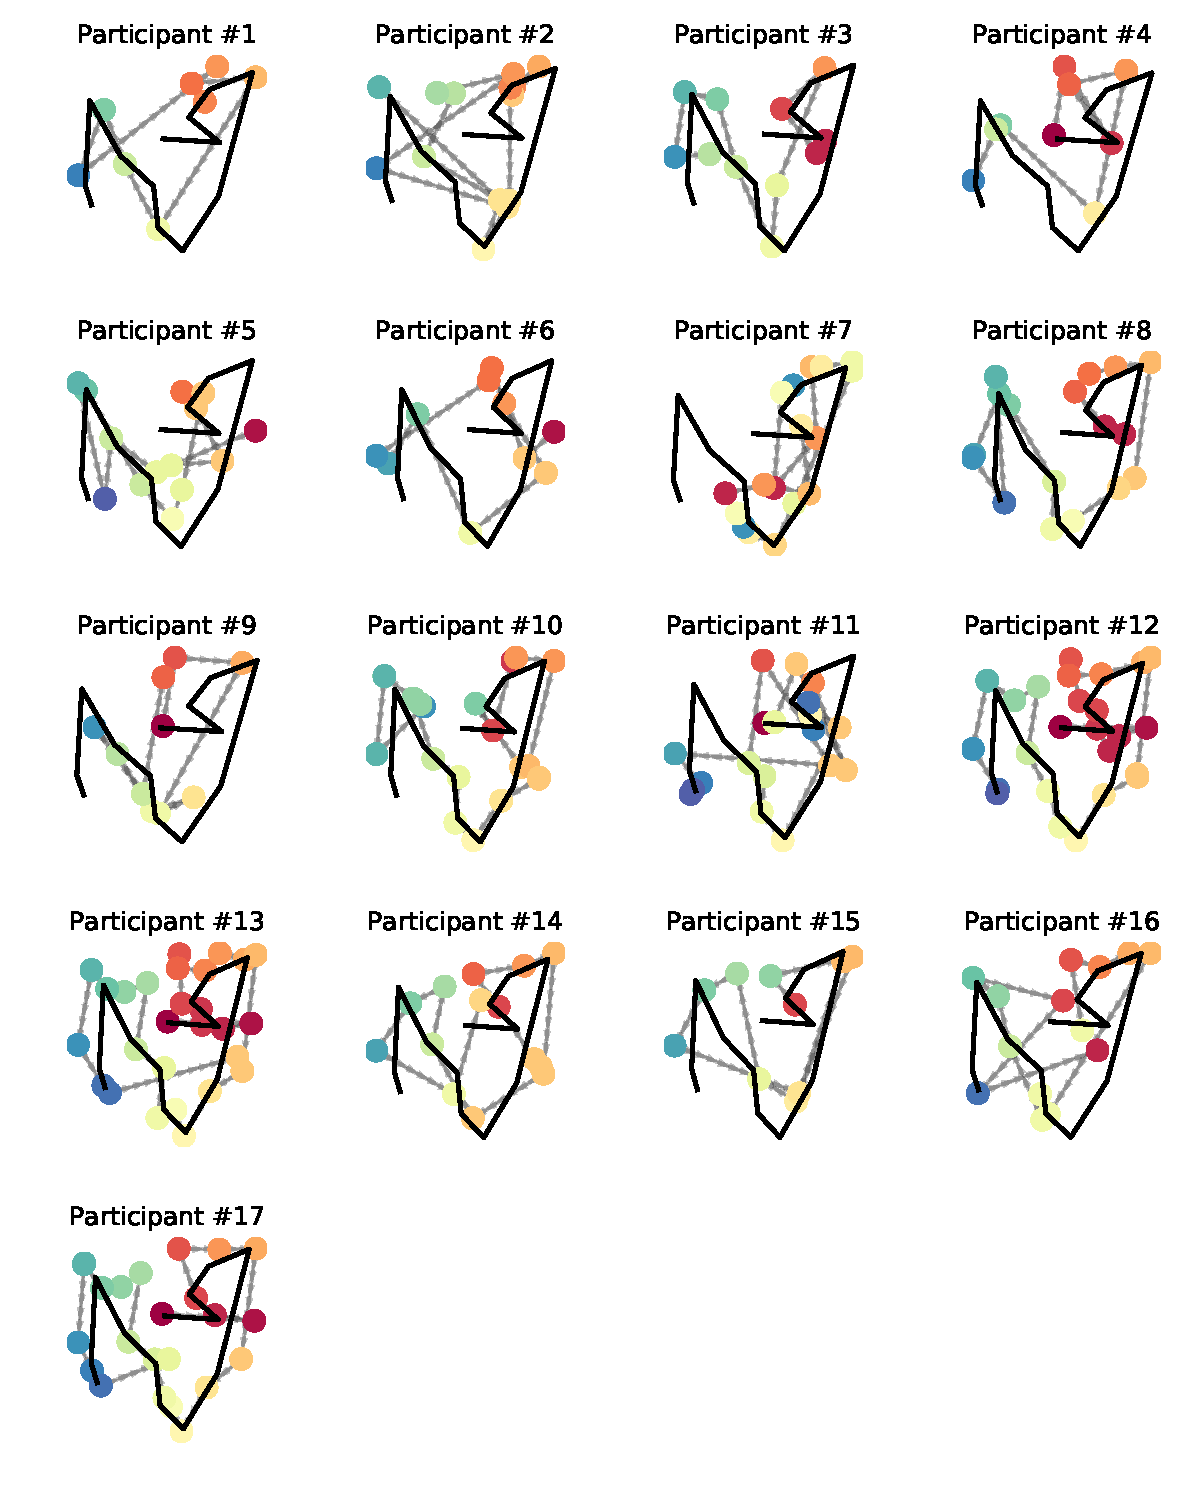
\includegraphics[width=1\textwidth]{figs/supp2_projs.pdf}
\caption{\small \textbf{Individual participant recall event model embeddings.} Each participant's recall event model embedded into a 2D space using the UMAP algorithm. The arrows on the lines connecting the recall events represents the direction of the sequence of recalls.  The color of the dots represent the most likely (i.e. most correlated) video event. The dark black line represents the best fitting line segment model (same for each participant).}
\label{fig:ind_embeddings}
\end{figure}
